\section{Details on Interpolation and Extrapolation} \label{appendix:methodology}

\noindent In the next lines, we provide details on the approach to estimate treatment effects. The difference in the approach for each outcome is based on different scenarios of data availability.

\subsection{Complete Data}
\label{app:method_fullobs}

\noindent  In the case where we have complete data, we only need to address compromised randomization. Appendix~\ref{appendix:assessingcc} shows that our estimates have little sensitivity to randomization compromises. Our baseline estimates throughout the paper do not account for this. By complete data, we mean that we observe the data for at least 90\% of the individuals in the sample. Table~\ref{table:nonipw} lists the variables that are completely observed.\\

\noindent For these outcomes, we estimate the standard errors of our estimates by resampling the ABC/CARE data. We estimate non-parametric $p$-values based on the bootstrap distribution. We perform inference in this same way throughout the paper.

\begin{table}[H]
\begin{threeparttable}
\caption{Variables Estimated without IPW Adjustment}
\label{table:nonipw}
\centering
% CONTENT CREATED ON SPREADSHEET, TREAT AS A .CSV (TAB DELIMITED)
% CAN BE COPIED INTO A SPREADSHEET PROGRAM (EXCEL, LIBRECALC) FOR EDITING
\begin{tabular}{l l}
\toprule
Variable	&	Age	\\
\midrule			
IQ Standard Score	&	2, 3, 4, 5, 6, 7, 8, 12, 15, 21	\\
PIAT Math Standard Score	&	7	\\
Home Total Score	&	0.5, 1.5, 2.5, 3.5, 4.5, 8	\\
Mother Works	&	2, 3, 4, 5	\\
Biological Mother's Education Level	&	2, 3, 4, 5, 9	\\
Father is Home	&	2, 3, 4, 5	\\
Ever Adopted	&		NA \\
Graduated High School	&	NA	\\
Attended Vocation/Tech/Community College	&	NA	\\
Earned Degree from 4-year College	&	NA	\\
Years of Education	&	30	\\
Works a Job	&	30	\\
Total Felony Arrests	&	Mid-30s	\\
Total Misdemeanor Arrests	&	Mid-30s	\\
Total Years Incarcerated	&	30	\\
Self-reported Health	&	30	\\
Number of Cigarettes Smoked Per Day Last Month	&	30	\\
Number of Days Drank Alcohol Last Month	&	30	\\
Number of Days Binge Drank Alcohol Last Month	&	30	\\
Program Costs	&	0--26	\\
Control Contamination Costs	&	0--26	\\
Education Costs	&	0--26	\\
Medical Expenditure &	8--30	\\
Justice System Costs	&	0--50	\\
Prison Costs	&	0--50	\\
Victimization Costs	&	0--50	\\
\bottomrule			
\end{tabular}
\begin{tablenotes}
\footnotesize
\item Note: The table above lists the variables for which we do not apply IPW when estimating
treatment effects.
\end{tablenotes}
\end{threeparttable}
\end{table}

\subsection{Partially Complete Data}
\label{app:method_partialobs}

\noindent When we do not observe data for more than 10\% of the individuals in the sample, we consider an outcome partially complete. These outcomes include: parental income at ages 2, 3, 4, 5, 9, 12, and 15, for which we observe no more than 91 subjects at any given age; and the health survey at age 34, for which we observe no more than 72 subjects.\\

\noindent For partially complete outcomes, we correct for attrition using an inverse probability scheme (IPW) as in  \citet{Horvitz_Thompson_1952_JASA}. To estimate the propensity to respond, we estimate a logit model of observing the outcome,
controlling for treatment status and three additional covariates. The additional covariates are
chosen among a set of variables, as detailed in Appendix~\ref{appendix:bvariables}. We account for the sampling variation implied in the estimation by the (IPW) scheme when producing our bootstrap-based inference.

\noindent \textbf{[JJH: Is this still valid?] [JLG: Yes. Please see Appendix~\ref{appendix:bvariables}. It contains the discussion on how we select control variables when estimating the IPW and when controlling for background variables when estimating treatment effects. The discussion on background variables to produce the forecasts is separate.]}\\

\subsection{Incomplete Data}
\label{app:method_noobs}

\noindent We do not observe life-cycle profiles for outcomes that are crucial to evaluate the effect of ABC/CARE. The three main examples are parental income, subject labor income, and public-transfer income. The importance of the first one is that ABC/CARE, in practice, had a childcare element. It relaxed the time constraints of the mothers of the treated children, who therefore were able to study or to work more. Potentially, this shifted the life-cycle profile of the mothers, either by allowing her to have more schooling or more working experience. We estimate these profiles. Similarly, a comprehensive evaluation accounts for the effect on the whole life-cycle profile of subject labor income and public-transfer income. We follow the strategy in Section~\ref{section:cbamethodology} to identify and estimate these profiles, i.e. to produce forecasts.

\subsubsection{Subject and Transfer Income}

\noindent Labor income and public-transfer income of subjects are only observed at ages 21 and 30.\footnote{At age 21, public-transfer income includes Aid to Families with Dependent Children (AFDC) subsidies, food stamps, survivor benefits, disability benefits, social security, rent subsidies, and fuel subsidies. At age 30, public-transfer income includes food stamps, welfare, housing assistance, workman's compensation, disability, social security, supplemental security income, unemployment benefits, worker's compensation insurance, fuel subsidies, educational and aid grants, and other forms of welfare.} For all other ages, we produce a forecast (either an interpolation or an extrapolation).

\subsubsection{Parental Income}

\noindent We use the same methodology to identify and estimate the life-cycle profile of parental income as the one we use for subject and transfer income. There is one difference to note. For subject and transfer income, we initialize the forecast at age 21 and go all the way to age 65---assumed age of retirement. For parental income, we initialize the forecast at age 0, in which we observe the outcome. For ages 2, 3, 4, 5, 9, 12, and 15 we do not use an estimate because we observe the data.

\textbf{[JJH: Jorge, can we not do better? Impute profiles using PSID?]}\textbf{[JLG: the reason for doing a linear interpolation is that the support in the PSID doesn't let us do much here. The information on the parents is not very complete. PSID of course surveys parents and children, but the matches here are adults and their parents barely appear in PSID. In other words, we are matching the ABC/CARE subjects to individuals who are not young enough as for us to obtain a good income profile of their parents.  We have eight observations between ages 0 and 15 and we are relying on that now.]} \textbf{[JJH: No, you are missing my point. Once the woman works she continues to work -at age 35 or so they have 25-30 years of work life left. Right now we underestimate parental income.] [JLG: I agree. I'm sorry for the confusion but the argument to follow up to age 15 only was other (that the child may not benefit from this given he might have moved out or so). The argument of women's wage growth was only recently brought up. I'm producing a forecast.]}\\

\subsection{Auxiliary Datasets and Variables Used to Forecast}

\subsubsection{Auxiliary Datasets}

\noindent We rely on the following datasets to estimate life-cycle profiles. We use this data in a very similar way to estimate the three life-cycle profiles of interest. For subject's labor income and parental labor income we use the exact same data. Two differences are: (i) for parental income, we need to produce a life-cycle profile from where the child is zero years old to when her mother is 65 (age at which we assume she retires); (ii) for parental income, we observe more years, and therefore need to produce a forecast for less time points.

\noindent A brief description of the auxiliary or non-experimental datasets and their use follows.\\

\noindent \textbf{The National Longitudinal Survey of Youth (NLSY79)} is a longitudinal survey beginning in 1979 that follows individuals born between 1957 and 1964. The initial interview included 12,686 respondents aged 14 to 22. The survey was designed to include 6,111 individuals representing the non-institutionalized civilian population, a supplemental sample of 5,295 civilian Hispanics, Latinos, blacks, non-blacks/non-Hispanics, and economically disadvantaged youth, and a sample of 1,280 who served in the military as of September 30, 1978. When appropriately weighted, the NLSY79 is nationally representative of the youth living in the U.S. on January 1, 1979. We include individuals from all three subsamples in our analysis. \\

\noindent The NLSY79 collected data on labor market participation, education, family background, family life, health issues, assets and income, government program participation, and measures of cognitive skills. We use these data for our estimation from ages 31 to 67.\\

\noindent We restrict the NLSY79 sample to individuals with labor income less than \$300,000 (2014 USD) at any given year. With the mean labor income (2014 USD) in the ABC/CARE sample being \$12,232 at age 21 and \$32,782 at age 30, and the maximum reported being \$189,938, the cut-off we impose on the auxiliary data is high enough so that everyone in the ABC/CARE sample is represented, yet low enough to exclude high-earning individuals in the auxiliary sample that do not reflect the ABC/CARE sample well. \\

\noindent We do not impose a restriction on birth year on the NLSY79 as all respondents are aged between 47 and 55 at the time of the last interview (conducted in 2012). This age range is within the 31--67 range for which we extrapolate the income of the ABC/CARE subjects. \\

\noindent Given the biennial nature of the NLSY79, we only observe each subject at either odd or even ages. Not only does this reduce the size of the sample on which we fit our prediction model at each age, but it can introduce biases associated with the odd-aged and even-aged cohorts. To address this issue, we perform a linear interpolation on the variables in the NLSY79 data that enter into our prediction model. This allows us to estimate our prediction model on all subjects of the NLSY79 satisfying our restrictions at every age. \\

\noindent \textbf{The Children of the National Longitudinal Survey of Youth (CNLSY)} is a survey of the children of the mothers from the NLSY, beginning in 1986. At the time of the initial interview, the ages of the children surveyed ranged from 0 to 23. As of 2010, the CNLSY sample includes 11,504 children born to NLSY79 mothers. With appropriate weights, the CNLSY may be considered nationally representative of children born to women who were aged 14 to 22 during 1979. Interviews were conducted annually between 1986 and 1994, and biennially thereafter. \\

\noindent Similar to the NLSY, the CNLSY collected data on cognitive ability, motor and social development, home environment, health information, education, attitudes, employment, income, family decisions, and more. We use these data to estimate a prediction model for subject income for ages 22 through 29. \\

\noindent As we did with the NLSY, we restrict the CNLSY sample to individuals with labor income less than \$300,000 (2014 USD) at any given year. In addition to this, we limit the sample to subjects born between 1978 and 1983. Because the CNLSY data extends to 2012, this implies that we use the most recent data from the CNLSY in which individuals are aged 29 to 34. Finally, given the biennial nature of the survey, we perform a linear interpolation on the variables that enter into our prediction model. This allows us to use as much of the CNLSY data as possible at every age when interpolating subject income. \\

\noindent \textbf{The Panel Survey of Income Dynamics (PSID)} is a longitudinal household survey containing between 5,000 and 8,500 families in each wave. It began as a yearly survey in 1968 and has been fielded biennially since 1996. When appropriately weighted, the PSID is designed to be representative of U.S. households. The PSID provides extensive information concerning demographics, economic outcomes, health outcomes, marriage and fertility, and more. In addition to using the PSID to forecast future earnings of ABC/CARE subjects, we use the PSID to forecast health outcomes. See Appendix \ref{section:data_psid} for details on how the PSID relates to health outcomes. \\

\noindent Similar to the CNLSY, we restrict the PSID to individuals born between 1945 and 1981. Because the data extend to 2013, we use the most recent subsample of individuals aged 30 to 67. We also exclude all individuals with labor income exceeding \$300,000 (2014 USD) in any given year. Finally, given the biennial nature of the survey, we perform a linear interpolation on the variables that enter into our prediction model. This allows us to use as much of the PSID data as possible at every age to interpolate subject income. \\

\subsubsection{Variables Used to Forecast}

\noindent We base our forecasts on three types of variables. We call $X,W,Z$ forecasting variables. Variables that could have not been affected by treatment, or pre-treatment variables. We divide these into two categories, pre-treatment variables used in the randomization protocol of ABC/CARE and pre-treatment variables not used in this protocol. We denote this by $Z$ and $W$, respectively. We let $X$ denote denote the variables that could have been affected by treatment.\\

\noindent At each age, our forecast is a function of the forecasting variables.\footnote{As we explain in the main paper, it is also possible to let our forecast in $t$ depend on our forecast in $t-1$. Suppose we want to forecast $Y_{t}$. We can base our forecast not only on $X,W,Z$ but also on our forecast of $Y_{t-1}$.} Our forecast is based on identifying and estimating a relationship between the outcome we want to forecast at time $t$, $Y_{t}$, in the non-experimental samples and then using this relationship in the experimental sample.\\

\noindent To be considered a forecasting variable, the variable must satisfy three restrictions: (i) it has to be available in the experimental and non-experimental samples; (ii) it has to have predictive power on the forecasted outcome; (iii) a common support assumption between the experimental and non-experimental datasets needs to be satisfied, as we formalize in Section~\ref{section:methodology}.\\

\noindent For a variable to satisfy restrictions (i) and (ii), it needs to be the case not only that the variable is available in the non-experimental sample but also that the survey question leading to it was introduced far enough back in time for us to observe it in a range that is common to the range in which we observe the variables in the experimental sample. To illustrate this, consider the case of body-mass index in the PSID. Survey questions leading to its availability were introduced in the late 1990s. The sample for whom the question was introduced, however, does not span enough observations for its support to cover the support of the experimental sample.\\

\noindent An alternative we follow to lower this problem is to pool diverse auxiliary datasets to cover the support in the experimental dataset.\\

\noindent The variables satisfying the first restriction are: indicator variables for being male and being black ($Z$); mother's education ($W$); PIAT scores at ages 5-7;\footnote{We take the average of the PIAT across ages 5 to 7. For ABC, we observe this variable. For CARE, we use the mathematics section of the Woodcock Johnson at these same ages because we do not observe PIAT.} years of education at age 30; labor income at ages 21 and 30; and BMI at age 34 ($X$). We provide tests for restrictions (i) and (ii) next and then discuss potential sensitivity to the choice of these variables.

\subsubsection{Common Support}

\noindent We \textbf{assume common support} between these auxiliary datasets and the analysis sample. This is required in order for us to reliably use external data to provide forecast for the ABC/CARE samples. Figure~\ref{fig:support} validates this assumption by displaying the overlapping support sets of ABC/CARE and our auxiliary data for the variables used to interpolate and extrapolate earnings.\footnote{For the male and black indicators, we do not provide evidence of common support. All three non-experimental samples have vast numbers of males, females, and black individuals to cover the support in the experimental samples.}\\

\begin{figure}[H]
		\caption{Support of ABC/CARE and Auxiliary Data} \label{fig:support}
	\begin{subfigure}[h]{0.8\textwidth}
	\centering
	\caption{Average PIAT Math Scores, Ages 5--7} \label{fig:support_math}
	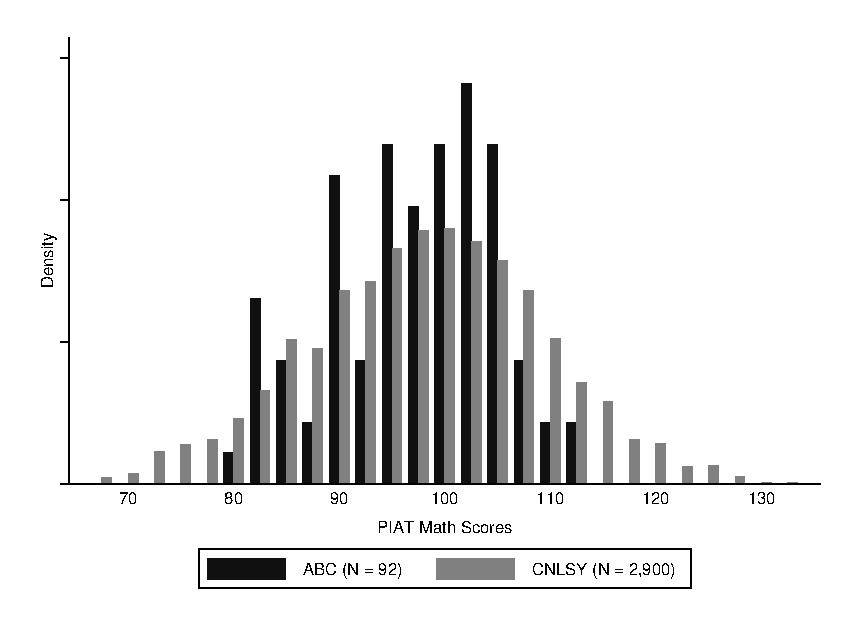
\includegraphics[width=\textwidth]{AppOutput/Methodology/support_math.eps}
	\end{subfigure}
	
	\begin{subfigure}[h]{0.8\textwidth}
	\centering
	\caption{Mother's Years of Education} \label{fig:support_meduc}
	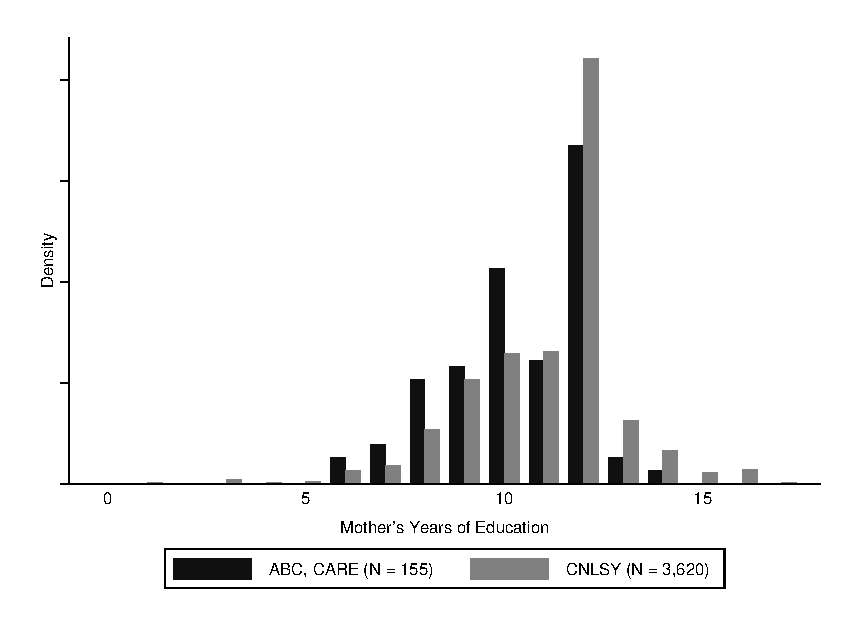
\includegraphics[width=\textwidth]{AppOutput/Methodology/support_momed.eps}
	\end{subfigure}
	
	\floatfoot{
	\footnotesize
	\noindent Note: These graphs display the support of ABC, PSID, NLSY79, and CNLSY
	for variables we use to project future earnings. PIAT math
	scores are averaged over ages 5--7.
	}
\end{figure}

\begin{figure}[H]
		\ContinuedFloat
	\begin{subfigure}[h]{0.8\textwidth}
	\centering
	\caption{Subject's Years of Education} \label{fig:support_educ}
	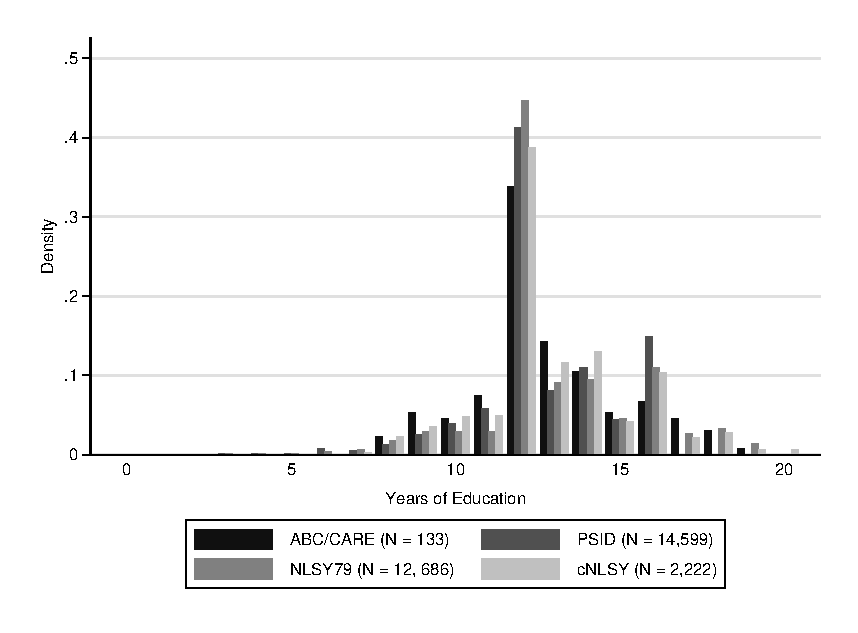
\includegraphics[width=\textwidth]{AppOutput/Methodology/support_educ.eps}
	\end{subfigure}
	
	\begin{subfigure}[h]{0.8\textwidth}
	\centering
	\caption{Income at Age 21} \label{fig:support_inc21}
	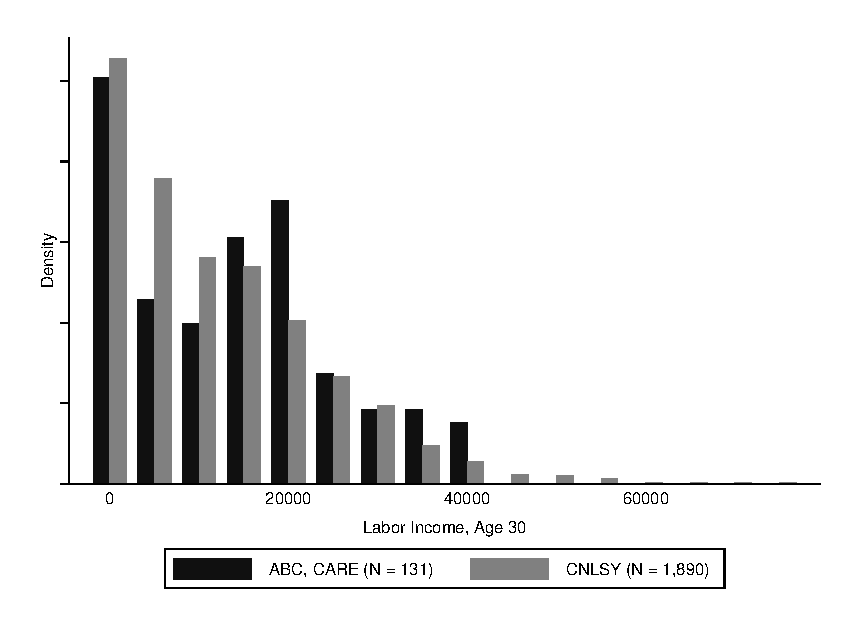
\includegraphics[width=\textwidth]{AppOutput/Methodology/support_inc21.eps}
	\end{subfigure}
	
\end{figure}

\begin{figure}[H]
	\ContinuedFloat
	
	\begin{subfigure}[h]{0.8\textwidth}
	\centering
	\caption{Income at Age 30} \label{fig:support_inc30}
	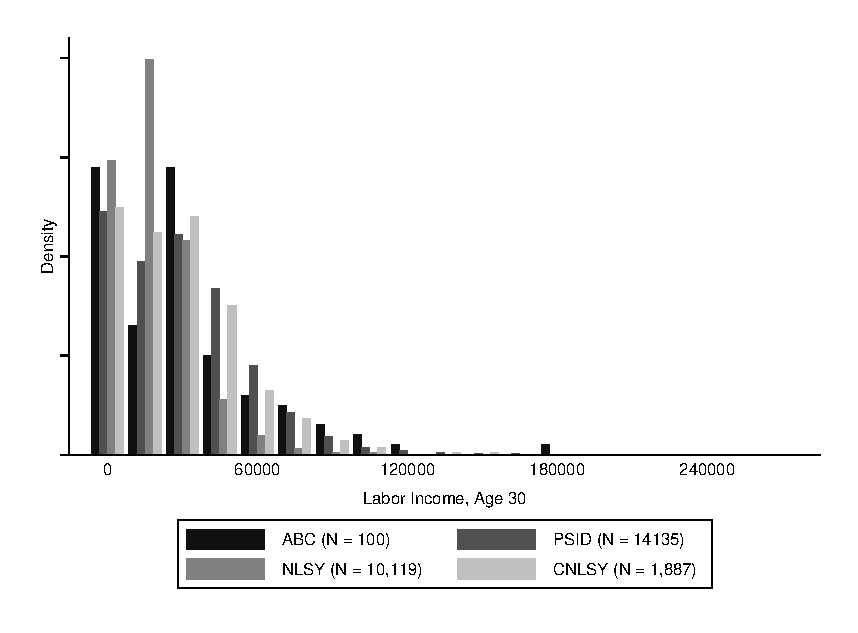
\includegraphics[width=\textwidth]{AppOutput/Methodology/support_inc30.eps}
	\end{subfigure}

	
	\begin{subfigure}[h]{0.8\textwidth}
	\centering
	\caption{Body Mass Index, Age 34} \label{fig:support_bmi}
	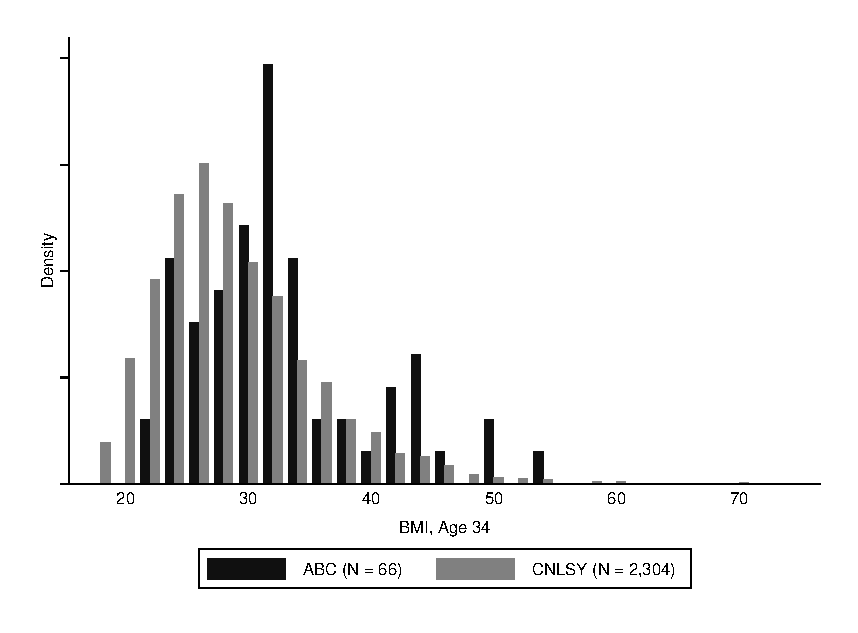
\includegraphics[width=\textwidth]{AppOutput/Methodology/support_bmi.eps}
	\end{subfigure}
	
\end{figure}

\subsubsection{Predictive Power}

\noindent We present evidence on the second restriction next. Tables~\ref{table:predpsid} to \ref{table:predcnlsy} show that, in each of the auxiliary samples that we use, the forecasting variables $X,W,Z$ are strong predictors of labor income at age 30. We present this evidence at age 30 both for brevity and to compare the predictive power of $X,W,Z$ on the outcomes we consider in the ABC/CARE sample.

\begin{table}[H] 
\begin{threeparttable}
\caption{Predictors of Labor Income at Age 30, PSID}
\label{table:predpsid}
\centering 
\begin{tabular}{lccc} \toprule
 & (1) & (2) & (3) \\ \midrule
Male & 19,877.340*** & 20,336.227*** & 7,686.820*** \\
 & (404.768) & (390.549) & (411.552) \\
Black & -9,761.792*** & -6,406.807*** & -1,793.755*** \\
 & (385.350) & (362.171) & (299.889) \\
Education (30)  &  & 4,109.973*** & 1,619.779*** \\
 &  & (91.929) & (92.105) \\
Labor Income (28) &  &  & 0.741*** \\
 &  &  & (0.014) \\
Cons & 23,953.099*** & -30,187.589*** & -14,016.536*** \\
 & (289.118) & (1,167.401) & (1,080.036) \\
 &  &  &  \\ \\ \midrule
Observations & 14,979 & 13,908 & 9,812 \\
$R^2$ & 0.172 & 0.291 & 0.657 \\ \bottomrule
\end{tabular}

\begin{tablenotes}
\footnotesize
\item Note: All columns display regressions of labor income at age 30 on the different variables listed in the rows. If the space for the coefficient appears empty, it was not included in the regression. All money figures are in 2014 USD. The parentheses next to the variable indicates the age of measurement. Education is measures as years of education. Robust standard errors are in parentheses. $^{***}$: $p$-value $< .01$. $^{**}$: $p$-value $< .05$. $^{*}$: $p$-value $< .10$.
\end{tablenotes}
\end{threeparttable}
\end{table}

\begin{table}[H] 
\begin{threeparttable}
\caption{Predictors of Labor Income at Age 30, NLSY79}
\label{table:prednlsy}
\centering 
\begin{tabular}{lcccccccc} \toprule
 & (1) & (2) & (3) & (4) & (5) & (6) & (7) & (8) \\
 Group Matched & Control & Treatment & Control & Treatment & Control & Treatment & Control & Treatment \\ \midrule
Male & 6,219.175*** & 6,356.307*** & 7,117.820*** & 7,607.672*** & 5,725.956*** & 6,216.821*** & 2,106.570*** & 2,311.490*** \\
 & (381.462) & (444.690) & (352.939) & (407.219) & (364.544) & (425.777) & (265.712) & (303.553) \\
Black & -5,607.642*** & -5,688.084*** & -5,150.394*** & -4,994.999*** & -3,823.029*** & -3,775.318*** & -1,737.614*** & -1,621.612*** \\
 & (386.635) & (439.804) & (356.854) & (399.225) & (381.924) & (431.636) & (256.122) & (287.850) \\
Education (30) &  &  & 2,536.795*** & 2,634.281*** & 2,593.961*** & 2,706.537*** & 799.974*** & 773.933*** \\
 &  &  & (81.757) & (95.205) & (85.765) & (100.476) & (73.768) & (79.358) \\
Labor Income (21) &  &  &  &  & 0.637*** & 0.627*** &  &  \\
 &  &  &  &  & (0.043) & (0.050) &  &  \\
Labor Income (28) &  &  &  &  &  &  & 0.774*** & 0.782*** \\
 &  &  &  &  &  &  & (0.021) & (0.022) \\
Constant & 15,572.398*** & 16,568.877*** & -17,659.060*** & -18,893.301*** & -21,611.129*** & -22,998.860*** & -5,761.074*** & -5,570.719*** \\
 & (304.541) & (336.484) & (1,085.558) & (1,274.381) & (1,148.548) & (1,366.048) & (834.721) & (959.266) \\ \\ \midrule Observations & 7,297 & 5,874 & 7,297 & 5,874 & 6,650 & 5,291 & 6,601 & 5,324 \\
$R^2$ & 0.102 & 0.095 & 0.245 & 0.250 & 0.309 & 0.305 & 0.690 & 0.693 \\ \hline
\end{tabular}

\begin{tablenotes}
\footnotesize
\item Note: Note: All columns display regressions of labor income at age 30 on the different variables listed in the rows. If the space for the coefficient appears empty, it was not included in the regression. All money figures are in 2014 USD. The parentheses next to the variable indicates the age of measurement. Education is measures as years of education. Robust standard errors are in parentheses. $^{***}$: $p$-value $< .01$. $^{**}$: $p$-value $< .05$. $^{*}$: $p$-value $< .10$.
\end{tablenotes}
\end{threeparttable}
\end{table}

\begin{table}[H] 
\begin{threeparttable}
\caption{Predictors of Labor Income at Age 30, CLSY}
\label{table:predcnlsy}
\centering 
\begin{tabular}{lcccccc} \toprule
 & (1) & (2) & (3) & (4) & (5) & (6) \\ 
Group Matched & Control & Treatment & Control & Treatment & Control & Treatment \\ \midrule
Male & 7,919.35*** & 7,755.32*** & 7,483.55*** & 7,472.02*** & 3,634.65*** & 3,740.61*** \\
 & (937.46) & (974.57) & (990.66) & (1,030.20) & (1,231.12) & (1,306.46) \\
Black  & -7,480.51*** & -7,721.48*** & -3,669.31*** & -3,799.02*** & -1,853.59 & -2,022.28* \\
 & (925.86) & (961.86) & (989.18) & (1,029.09) & (1,156.85) & (1,202.94) \\
Mother's Education & 1,888.32*** & 1,833.29*** & 303.02 & 288.90 & 284.94 & 235.17 \\
 & (258.71) & (271.05) & (293.84) & (309.08) & (357.69) & (393.81) \\
PIAT (5-7) &  &  & 168.64*** & 170.88*** & 169.51*** & 169.89** \\
 &  &  & (48.44) & (50.18) & (63.42) & (66.41) \\
Education (30)  &  &  & 3,678.09*** & 3,736.28*** & 2,223.04*** & 2,353.75*** \\
 &  &  & (250.08) & (264.84) & (434.21) & (457.65) \\
Labor Income (21) &  &  & 0.51*** & 0.50*** &  &  \\
 &  &  & (0.06) & (0.06) &  &  \\
BMI (34) &  &  & -45.78 & -48.11 & -174.13* & -183.16* \\
 &  &  & (70.83) & (72.79) & (96.27) & (100.26) \\
Labor Income (28) &  &  &  &  & 0.48*** & 0.46*** \\
 &  &  &  &  & (0.07) & (0.07) \\
Constant & 4,170.58 & 5,151.64* & -47,898.77*** & -48,608.54*** & -30,593.81*** & -31,042.44*** \\
 & (2,940.08) & (3,083.88) & (5,285.02) & (5,504.80) & (6,818.91) & (7,102.58) \\ \\ \midrule
 Observations & 1,880 & 1,876 & 1,463 & 1,459 & 734 & 733 \\ 
$R^2$ & 0.09 & 0.09 & 0.29 & 0.29 & 0.50 & 0.49 \\ \bottomrule
\end{tabular}

\begin{tablenotes}
\footnotesize
\item Note: All columns display regressions of labor income at age 30 on the different variables listed in the rows. If the space for the coefficient appears empty, it was not included in the regression. All money figures are in 2014 USD. The parentheses next to the variable indicates the age of measurement. Education is measures as years of education. BMI stands for body-mass index. PIAT (5-7) is the average of the PIAT mathematics score from ages 5 to 7. Robust standard errors are in parentheses. $^{***}$: $p$-value $< .01$. $^{**}$: $p$-value $< .05$. $^{*}$: $p$-value $< .10$.
\end{tablenotes}
\end{threeparttable}
\end{table}

\begin{table}[H] 
\begin{threeparttable}
\caption{Predictors of Labor Income at Age 30, ABC/CARE}
\label{table:predabc}
\centering 
\begin{tabular}{lcc} \toprule
 & (1) & (2) \\ \midrule
Male & 15,127.641* & -624.472 \\
 & (7,850.718) & (5,384.686) \\
Mother's Education & 2,136.666 & -3,390.346 \\
 & (2,151.633) & (2,246.745) \\
PIAT (5-7) &  & -37.091 \\
 &  & (389.874) \\
Education (30) &  & 10,107.368*** \\
 &  & (3,777.647) \\
Labor Income (21) &  & 0.270 \\
 &  & (0.296) \\
BMI (34) &  & -320.535 \\
 &  & (241.455) \\
Cons & 2,165.045 & -52,896.960 \\
 & (23,054.657) & (32,236.828) \\
 &  &  \\ \\ \midrule
Observations & 132 & 76 \\
$R^2$ & 0.035 & 0.312 \\ \bottomrule
\end{tabular}

\begin{tablenotes}
\footnotesize
\item Note: Note: All columns display regressions of labor income at age 30 on the different variables listed in the rows. If the space for the coefficient appears empty, it was not included in the regression. All money figures are in 2014 USD. The parentheses next to the variable indicates the age of measurement. Education is measures as years of education. BMI stands for body-mass index. PIAT (5-7) is the average of the PIAT mathematics score from ages 5 to 7. For CARE children, we use the mathematics section of the Woodcock Johnson at these same ages because we do not observe PIAT Robust standard errors are in parentheses. $^{***}$: $p$-value $< .01$. $^{**}$: $p$-value $< .05$. $^{*}$: $p$-value $< .10$.
\end{tablenotes}
\end{threeparttable}
\end{table}

%%%%

\begin{table}[H] 
\begin{threeparttable}
\caption{Predictors of Transfer Income at Age 30, PSID}
\label{table:predpsid}
\centering 
\begin{tabular}{lccc} \toprule
 & (1) & (2) & (3) \\ \midrule
Male & 19,877.340*** & 20,336.227*** & 7,686.820*** \\
 & (404.768) & (390.549) & (411.552) \\
Black & -9,761.792*** & -6,406.807*** & -1,793.755*** \\
 & (385.350) & (362.171) & (299.889) \\
Education (30)  &  & 4,109.973*** & 1,619.779*** \\
 &  & (91.929) & (92.105) \\
Labor Income (28) &  &  & 0.741*** \\
 &  &  & (0.014) \\
Cons & 23,953.099*** & -30,187.589*** & -14,016.536*** \\
 & (289.118) & (1,167.401) & (1,080.036) \\
 &  &  &  \\ \\ \midrule
Observations & 14,979 & 13,908 & 9,812 \\
$R^2$ & 0.172 & 0.291 & 0.657 \\ \bottomrule
\end{tabular}

\begin{tablenotes}
\footnotesize
\item Note: All columns display regressions of transfer income at age 30 on the different variables listed in the rows. If the space for the coefficient appears empty, it was not included in the regression. All money figures are in 2014 USD. The parentheses next to the variable indicates the age of measurement. Education is measures as years of education. Robust standard errors are in parentheses. $^{***}$: $p$-value $< .01$. $^{**}$: $p$-value $< .05$. $^{*}$: $p$-value $< .10$.
\end{tablenotes}
\end{threeparttable}
\end{table}

\begin{table}[H] 
\begin{threeparttable}
\caption{Predictors of Transfer Income at Age 30, NLSY79}
\label{table:prednlsy}
\centering 
\begin{tabular}{lcccccccc} \toprule
 & (1) & (2) & (3) & (4) & (5) & (6) & (7) & (8) \\
 Group Matched & Control & Treatment & Control & Treatment & Control & Treatment & Control & Treatment \\ \midrule
Male & 6,219.175*** & 6,356.307*** & 7,117.820*** & 7,607.672*** & 5,725.956*** & 6,216.821*** & 2,106.570*** & 2,311.490*** \\
 & (381.462) & (444.690) & (352.939) & (407.219) & (364.544) & (425.777) & (265.712) & (303.553) \\
Black & -5,607.642*** & -5,688.084*** & -5,150.394*** & -4,994.999*** & -3,823.029*** & -3,775.318*** & -1,737.614*** & -1,621.612*** \\
 & (386.635) & (439.804) & (356.854) & (399.225) & (381.924) & (431.636) & (256.122) & (287.850) \\
Education (30) &  &  & 2,536.795*** & 2,634.281*** & 2,593.961*** & 2,706.537*** & 799.974*** & 773.933*** \\
 &  &  & (81.757) & (95.205) & (85.765) & (100.476) & (73.768) & (79.358) \\
Labor Income (21) &  &  &  &  & 0.637*** & 0.627*** &  &  \\
 &  &  &  &  & (0.043) & (0.050) &  &  \\
Labor Income (28) &  &  &  &  &  &  & 0.774*** & 0.782*** \\
 &  &  &  &  &  &  & (0.021) & (0.022) \\
Constant & 15,572.398*** & 16,568.877*** & -17,659.060*** & -18,893.301*** & -21,611.129*** & -22,998.860*** & -5,761.074*** & -5,570.719*** \\
 & (304.541) & (336.484) & (1,085.558) & (1,274.381) & (1,148.548) & (1,366.048) & (834.721) & (959.266) \\ \\ \midrule Observations & 7,297 & 5,874 & 7,297 & 5,874 & 6,650 & 5,291 & 6,601 & 5,324 \\
$R^2$ & 0.102 & 0.095 & 0.245 & 0.250 & 0.309 & 0.305 & 0.690 & 0.693 \\ \hline
\end{tabular}

\begin{tablenotes}
\footnotesize
\item Note: Note: All columns display regressions of transfer income at age 30 on the different variables listed in the rows. If the space for the coefficient appears empty, it was not included in the regression. All money figures are in 2014 USD. The parentheses next to the variable indicates the age of measurement. Education is measures as years of education. Robust standard errors are in parentheses. $^{***}$: $p$-value $< .01$. $^{**}$: $p$-value $< .05$. $^{*}$: $p$-value $< .10$.
\end{tablenotes}
\end{threeparttable}
\end{table}

\begin{table}[H] 
\begin{threeparttable}
\caption{Predictors of Transfer Income at Age 30, CLSY}
\label{table:predcnlsy}
\centering 
\begin{tabular}{lcccccc} \toprule
 & (1) & (2) & (3) & (4) & (5) & (6) \\ 
Group Matched & Control & Treatment & Control & Treatment & Control & Treatment \\ \midrule
Male & 7,919.35*** & 7,755.32*** & 7,483.55*** & 7,472.02*** & 3,634.65*** & 3,740.61*** \\
 & (937.46) & (974.57) & (990.66) & (1,030.20) & (1,231.12) & (1,306.46) \\
Black  & -7,480.51*** & -7,721.48*** & -3,669.31*** & -3,799.02*** & -1,853.59 & -2,022.28* \\
 & (925.86) & (961.86) & (989.18) & (1,029.09) & (1,156.85) & (1,202.94) \\
Mother's Education & 1,888.32*** & 1,833.29*** & 303.02 & 288.90 & 284.94 & 235.17 \\
 & (258.71) & (271.05) & (293.84) & (309.08) & (357.69) & (393.81) \\
PIAT (5-7) &  &  & 168.64*** & 170.88*** & 169.51*** & 169.89** \\
 &  &  & (48.44) & (50.18) & (63.42) & (66.41) \\
Education (30)  &  &  & 3,678.09*** & 3,736.28*** & 2,223.04*** & 2,353.75*** \\
 &  &  & (250.08) & (264.84) & (434.21) & (457.65) \\
Labor Income (21) &  &  & 0.51*** & 0.50*** &  &  \\
 &  &  & (0.06) & (0.06) &  &  \\
BMI (34) &  &  & -45.78 & -48.11 & -174.13* & -183.16* \\
 &  &  & (70.83) & (72.79) & (96.27) & (100.26) \\
Labor Income (28) &  &  &  &  & 0.48*** & 0.46*** \\
 &  &  &  &  & (0.07) & (0.07) \\
Constant & 4,170.58 & 5,151.64* & -47,898.77*** & -48,608.54*** & -30,593.81*** & -31,042.44*** \\
 & (2,940.08) & (3,083.88) & (5,285.02) & (5,504.80) & (6,818.91) & (7,102.58) \\ \\ \midrule
 Observations & 1,880 & 1,876 & 1,463 & 1,459 & 734 & 733 \\ 
$R^2$ & 0.09 & 0.09 & 0.29 & 0.29 & 0.50 & 0.49 \\ \bottomrule
\end{tabular}

\begin{tablenotes}
\footnotesize
\item Note: All columns display regressions of transfer income at age 30 on the different variables listed in the rows. If the space for the coefficient appears empty, it was not included in the regression. All money figures are in 2014 USD. The parentheses next to the variable indicates the age of measurement. Education is measures as years of education. BMI stands for body-mass index. PIAT (5-7) is the average of the PIAT mathematics score from ages 5 to 7. Robust standard errors are in parentheses. $^{***}$: $p$-value $< .01$. $^{**}$: $p$-value $< .05$. $^{*}$: $p$-value $< .10$.
\end{tablenotes}
\end{threeparttable}
\end{table}

\begin{table}[H] 
\begin{threeparttable}
\caption{Predictors of Transfer Income at Age 30, ABC/CARE}
\label{table:predabc}
\centering 
\begin{tabular}{lcc} \toprule
 & (1) & (2) \\ \midrule
Male & 15,127.641* & -624.472 \\
 & (7,850.718) & (5,384.686) \\
Mother's Education & 2,136.666 & -3,390.346 \\
 & (2,151.633) & (2,246.745) \\
PIAT (5-7) &  & -37.091 \\
 &  & (389.874) \\
Education (30) &  & 10,107.368*** \\
 &  & (3,777.647) \\
Labor Income (21) &  & 0.270 \\
 &  & (0.296) \\
BMI (34) &  & -320.535 \\
 &  & (241.455) \\
Cons & 2,165.045 & -52,896.960 \\
 & (23,054.657) & (32,236.828) \\
 &  &  \\ \\ \midrule
Observations & 132 & 76 \\
$R^2$ & 0.035 & 0.312 \\ \bottomrule
\end{tabular}

\begin{tablenotes}
\footnotesize
\item Note: Note: All columns display regressions of transfer income at age 30 on the different variables listed in the rows. If the space for the coefficient appears empty, it was not included in the regression. All money figures are in 2014 USD. The parentheses next to the variable indicates the age of measurement. Education is measures as years of education. BMI stands for body-mass index. PIAT (5-7) is the average of the PIAT mathematics score from ages 5 to 7. For CARE children, we use the mathematics section of the Woodcock Johnson at these same ages because we do not observe PIAT Robust standard errors are in parentheses. $^{***}$: $p$-value $< .01$. $^{**}$: $p$-value $< .05$. $^{*}$: $p$-value $< .10$.
\end{tablenotes}
\end{threeparttable}
\end{table}

\subsubsection{Sensitivity Analysis}

\noindent An immediate route of inquiry is the sensitivity of our forecasts to the use of different forecasting variables. We reproduce three exercises to analyze this for labor income: (i) our baseline forecast, which is based on $X,W,Z$ and the lagged value of the forecasted labor income, i.e. at time $t$ we base the forecast on $X,W,Z$ and (forecasted) labor income at $t-1$; (ii) the same as (i) but without using lagged labor income; (iii) the same as (i) but without using $X$; (iv) a forecast based exclusively on $W,Z$; (v) a forecast based exclusively on $X$.\\

\noindent Although the forecast in (i) is the most accurate if compared to low-skilled individuals in the PSID, they are robust to sensitivity analysis.\footnote{We obtain similar results exercises for transfer income and parental labor income and they are available under request.}

\begin{sidewaysfigure}[!htbp]
\centering
\caption{Labor Income Profiles, Forecast Based on Lageed Labor Income and $X,W,Z$}\label{fig:labor-income-profiles}
\begin{subfigure}[h]{0.4\textwidth}
		\centering
		\caption{Forecasted for ABC/CARE Males} \label{fig:abcare1}
		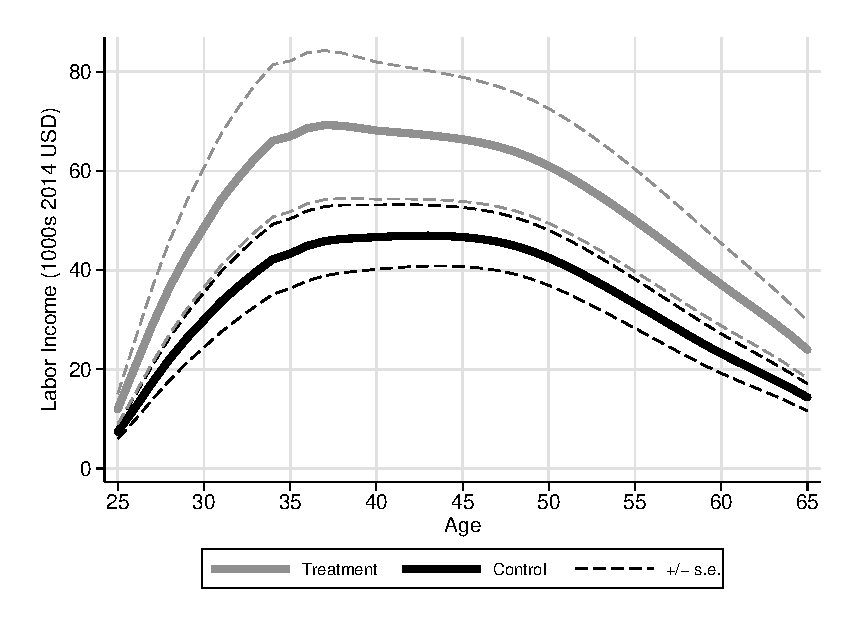
\includegraphics[width=\textwidth]{output/labor_25-60_male_1.eps}
\end{subfigure}%
\begin{subfigure}[h]{0.4\textwidth}
	\centering
	\caption{PSID, Disadvantaged Males} \label{fig:psid1}
		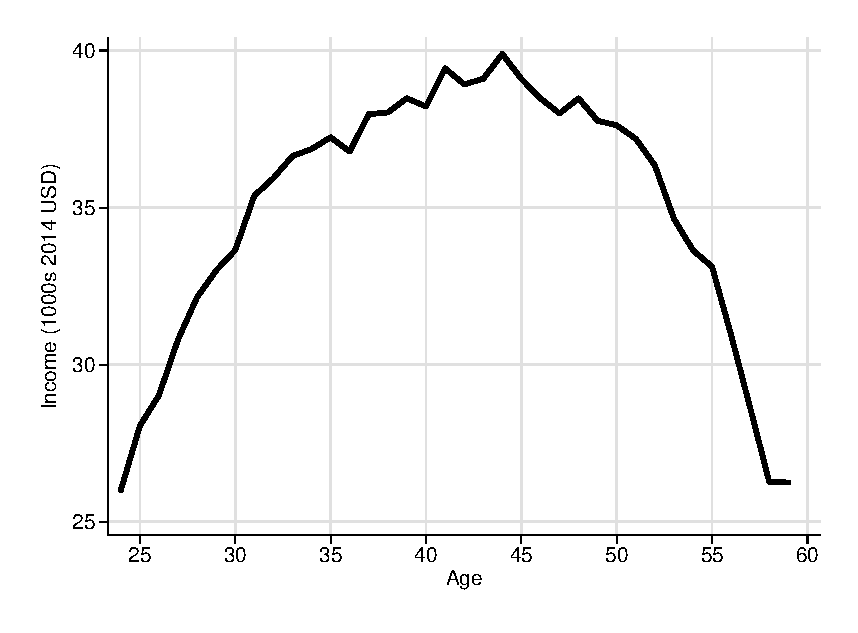
\includegraphics[width=\textwidth]{output/psid_incomeprofiles_s1.eps}
\end{subfigure}
\begin{subfigure}[h]{0.4\textwidth}
		\centering
		\caption{Forecasted for ABC/CARE Females} \label{fig:abcare0}
		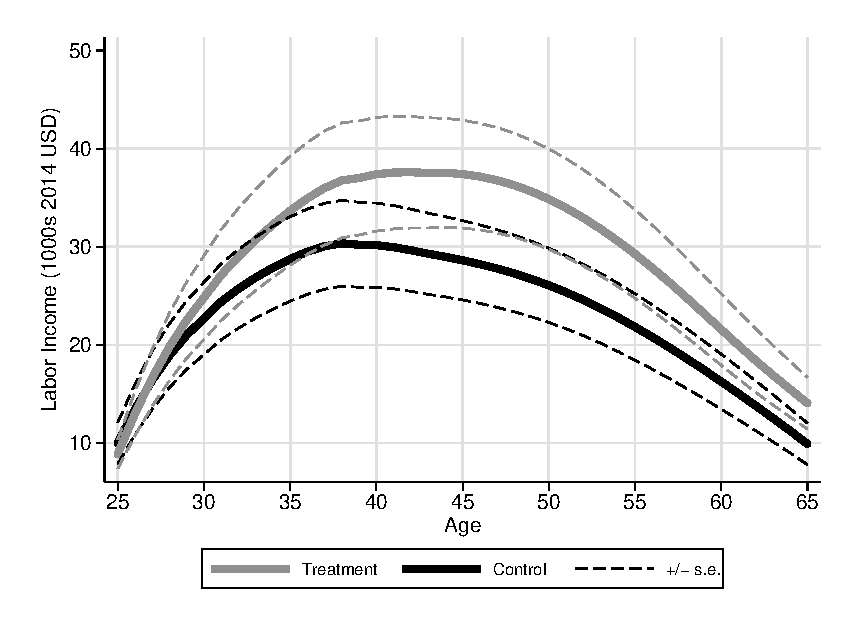
\includegraphics[width=\textwidth]{output/labor_25-60_female_1.eps}
\end{subfigure}%
\begin{subfigure}[h]{0.4\textwidth}
	\centering
	\caption{PSID, Disadvantaged Females} \label{fig:psid0}
		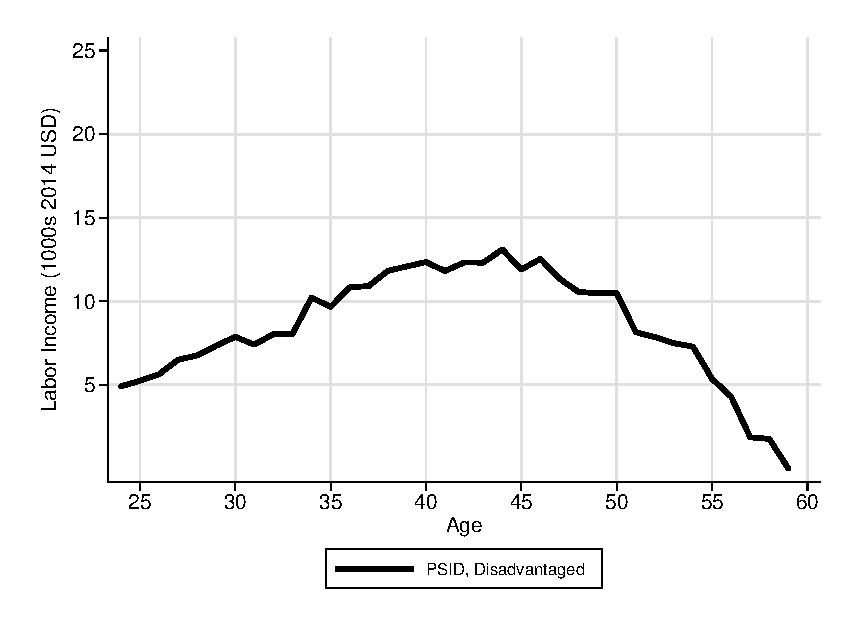
\includegraphics[width=\textwidth]{output/psid_incomeprofiles_s0.eps}
\end{subfigure}
\footnotesize \justify
Note: Panels (a) and (c) display the forecasted labor income profiles for ABC/CARE males and females by treatment status, based on forecasts that combine data from the Panel Study of Income Dynamics (PSID), the National Longitudinal Survey of Youth 1979 (NLSY79), and the Children of the National Longitudinal Survey of Youth 1979 (CNLSY79). Panels (b) and (d) display the mean labor income profile of disadvantaged males and females in the Panel Study of Income Dynamics (PSID), where disadvantaged is defined as having 12 years of education or less.\\
\end{sidewaysfigure}

\begin{sidewaysfigure}[!htbp]
\centering
\caption{Labor Income Profiles, Forecast Based on $X,W,Z$}\label{fig:labor-income-profiles}
\begin{subfigure}[h]{0.4\textwidth}
		\centering
		\caption{Forecasted for ABC/CARE Males} \label{fig:abcare1}
		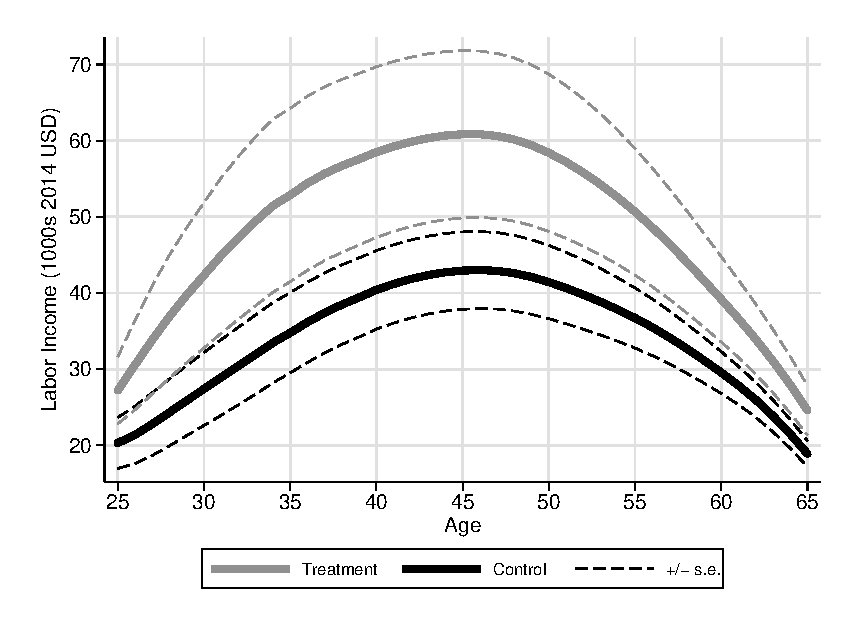
\includegraphics[width=\textwidth]{output/labor_25-60_male_2.eps}
\end{subfigure}%
\begin{subfigure}[h]{0.4\textwidth}
	\centering
	\caption{PSID, Disadvantaged Males} \label{fig:psid1}
		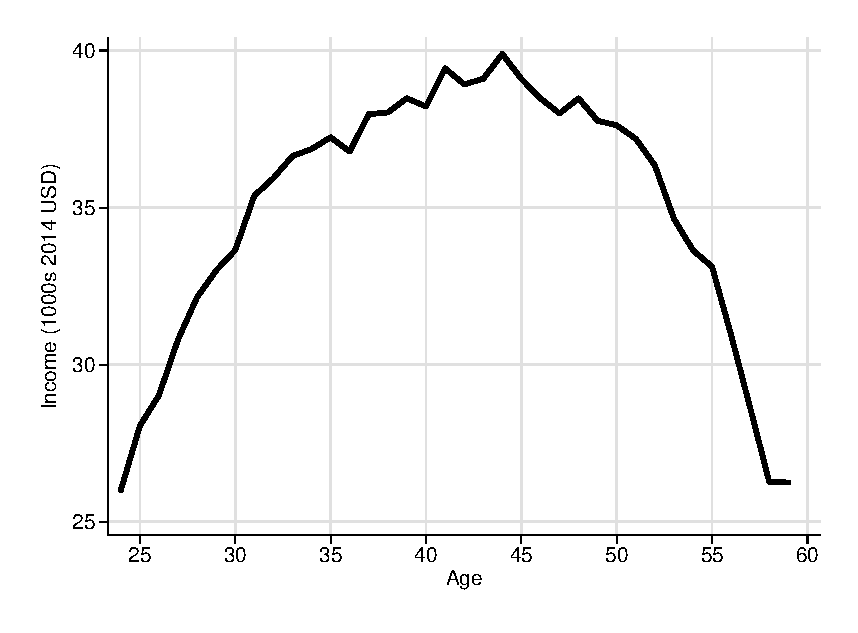
\includegraphics[width=\textwidth]{output/psid_incomeprofiles_s1.eps}
\end{subfigure}
\begin{subfigure}[h]{0.4\textwidth}
		\centering
		\caption{Forecasted for ABC/CARE Females} \label{fig:abcare0}
		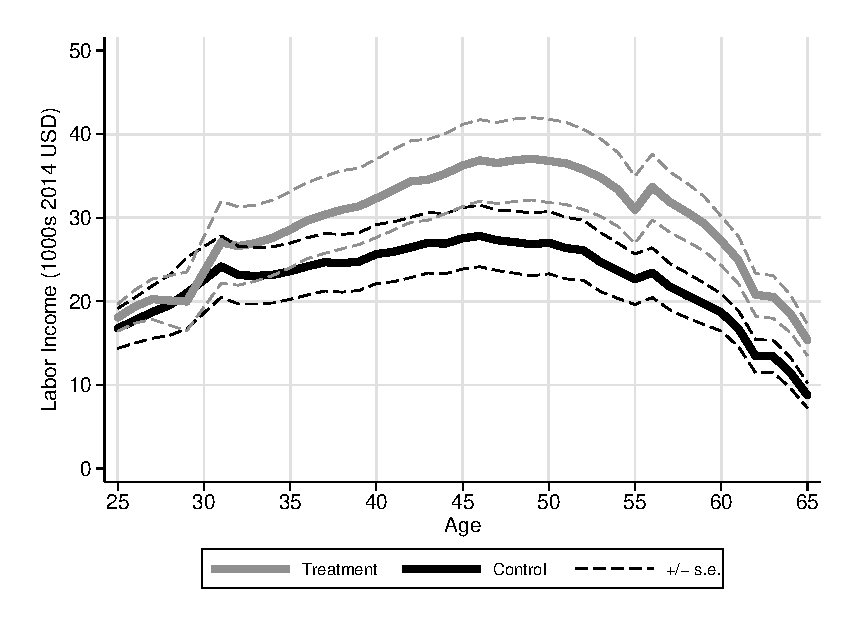
\includegraphics[width=\textwidth]{output/labor_25-60_female_2.eps}
\end{subfigure}%
\begin{subfigure}[h]{0.4\textwidth}
	\centering
	\caption{PSID, Disadvantaged Females} \label{fig:psid0}
		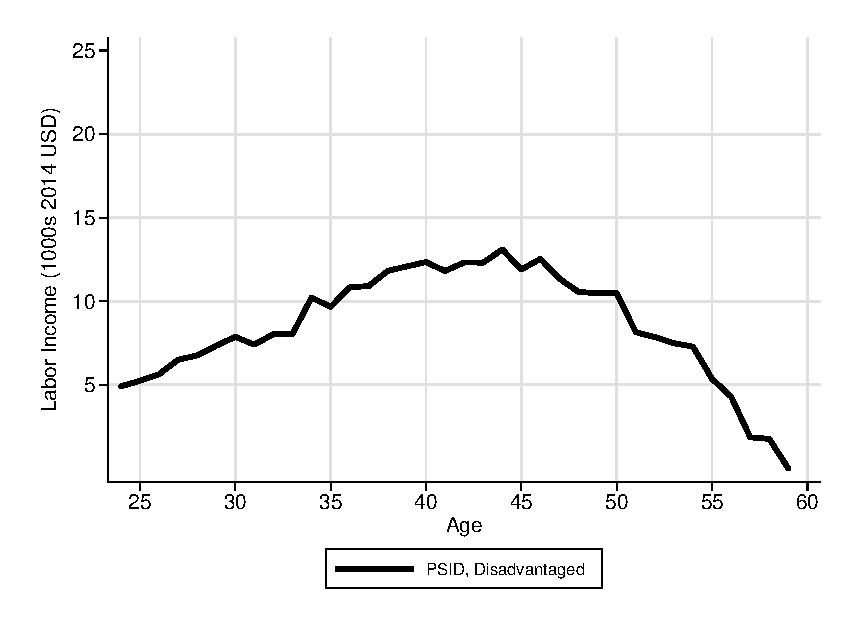
\includegraphics[width=\textwidth]{output/psid_incomeprofiles_s0.eps}
\end{subfigure}
\footnotesize \justify
Note: Panels (a) and (c) display the forecasted labor income profiles for ABC/CARE males and females by treatment status, based on forecasts that combine data from the Panel Study of Income Dynamics (PSID), the National Longitudinal Survey of Youth 1979 (NLSY79), and the Children of the National Longitudinal Survey of Youth 1979 (CNLSY79). Panels (b) and (d) display the mean labor income profile of disadvantaged males and females in the Panel Study of Income Dynamics (PSID), where disadvantaged is defined as having 12 years of education or less.\\
\end{sidewaysfigure}

\begin{sidewaysfigure}[!htbp]
\centering
\caption{Labor Income Profiles, Forecast Based on Lageed Labor Income and $W,Z$}\label{fig:labor-income-profiles}
\begin{subfigure}[h]{0.4\textwidth}
		\centering
		\caption{Forecasted for ABC/CARE Males} \label{fig:abcare1}
		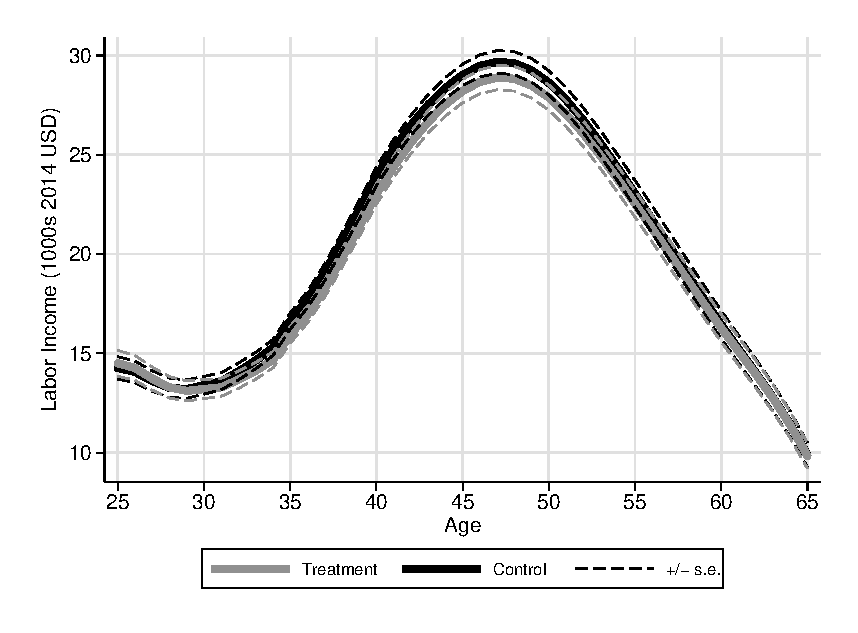
\includegraphics[width=\textwidth]{output/labor_25-60_male_3.eps}
\end{subfigure}%
\begin{subfigure}[h]{0.4\textwidth}
	\centering
	\caption{PSID, Disadvantaged Males} \label{fig:psid1}
		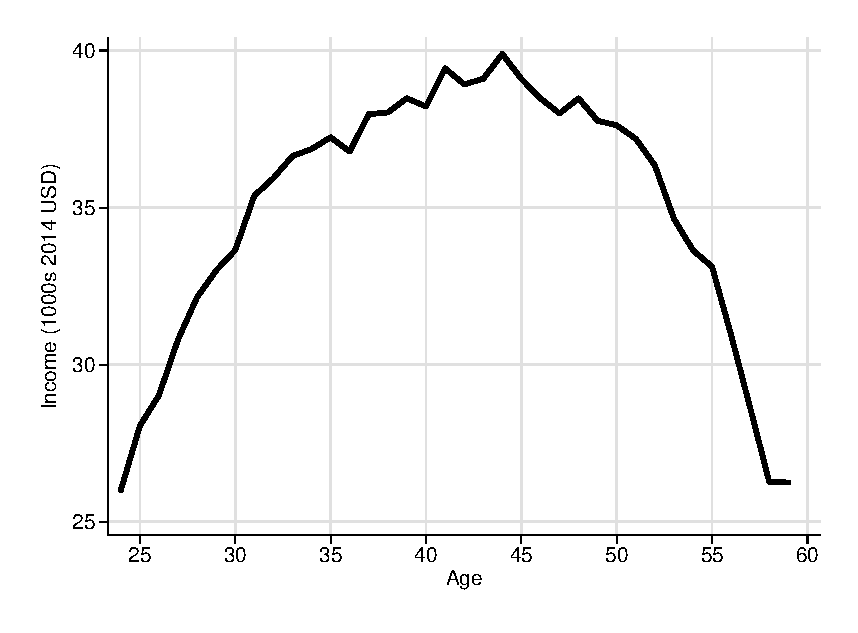
\includegraphics[width=\textwidth]{output/psid_incomeprofiles_s1.eps}
\end{subfigure}
\begin{subfigure}[h]{0.4\textwidth}
		\centering
		\caption{Forecasted for ABC/CARE Females} \label{fig:abcare0}
		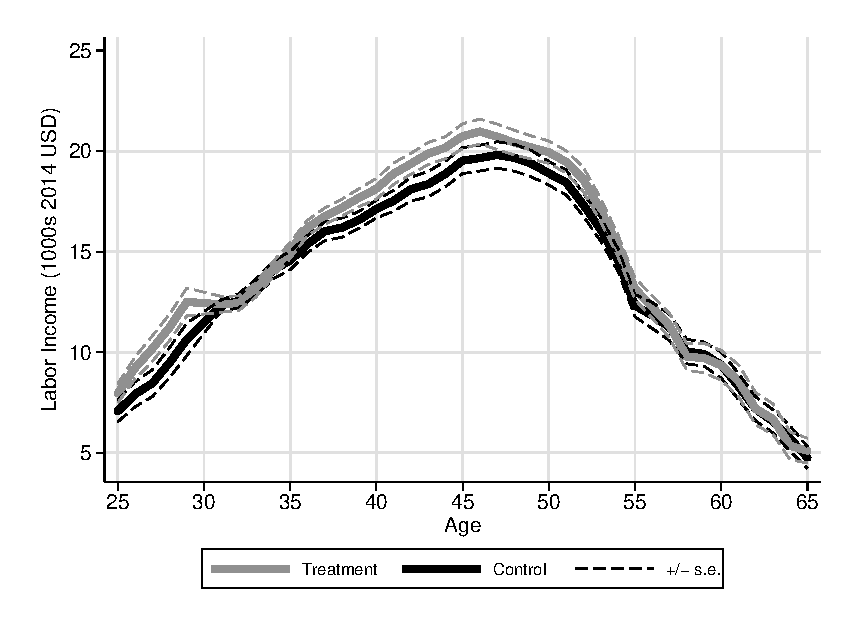
\includegraphics[width=\textwidth]{output/labor_25-60_female_3.eps}
\end{subfigure}%
\begin{subfigure}[h]{0.4\textwidth}
	\centering
	\caption{PSID, Disadvantaged Females} \label{fig:psid0}
		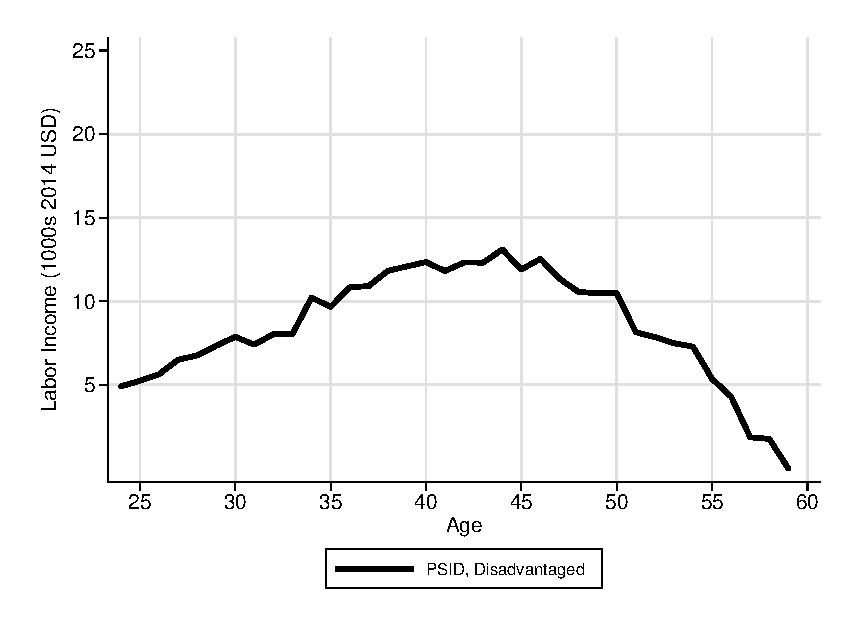
\includegraphics[width=\textwidth]{output/psid_incomeprofiles_s0.eps}
\end{subfigure}
\footnotesize \justify
Note: Panels (a) and (c) display the forecasted labor income profiles for ABC/CARE males and females by treatment status, based on forecasts that combine data from the Panel Study of Income Dynamics (PSID), the National Longitudinal Survey of Youth 1979 (NLSY79), and the Children of the National Longitudinal Survey of Youth 1979 (CNLSY79). Panels (b) and (d) display the mean labor income profile of disadvantaged males and females in the Panel Study of Income Dynamics (PSID), where disadvantaged is defined as having 12 years of education or less.\\
\end{sidewaysfigure}

\begin{sidewaysfigure}[!htbp]
\centering
\caption{Labor Income Profiles, Forecast Based $X$}\label{fig:labor-income-profiles}
\begin{subfigure}[h]{0.4\textwidth}
		\centering
		\caption{Forecasted for ABC/CARE Males} \label{fig:abcare1}
		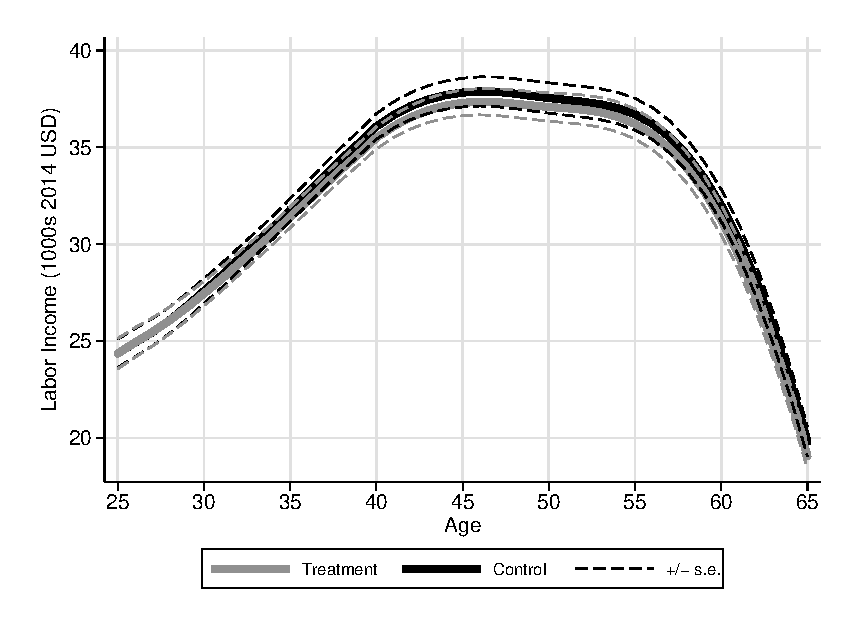
\includegraphics[width=\textwidth]{output/labor_25-60_male_4.eps}
\end{subfigure}%
\begin{subfigure}[h]{0.4\textwidth}
	\centering
	\caption{PSID, Disadvantaged Males} \label{fig:psid1}
		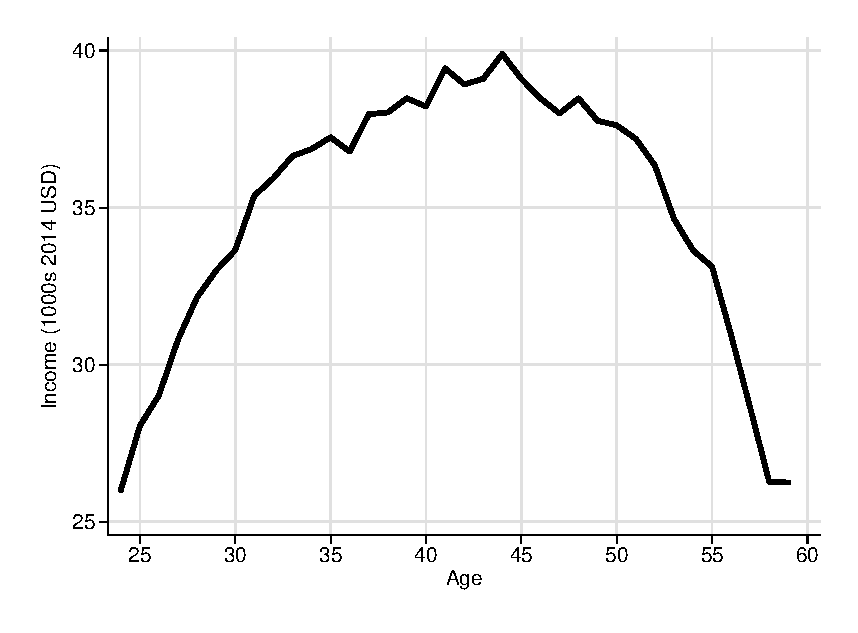
\includegraphics[width=\textwidth]{output/psid_incomeprofiles_s1.eps}
\end{subfigure}
\begin{subfigure}[h]{0.4\textwidth}
		\centering
		\caption{Forecasted for ABC/CARE Females} \label{fig:abcare0}
		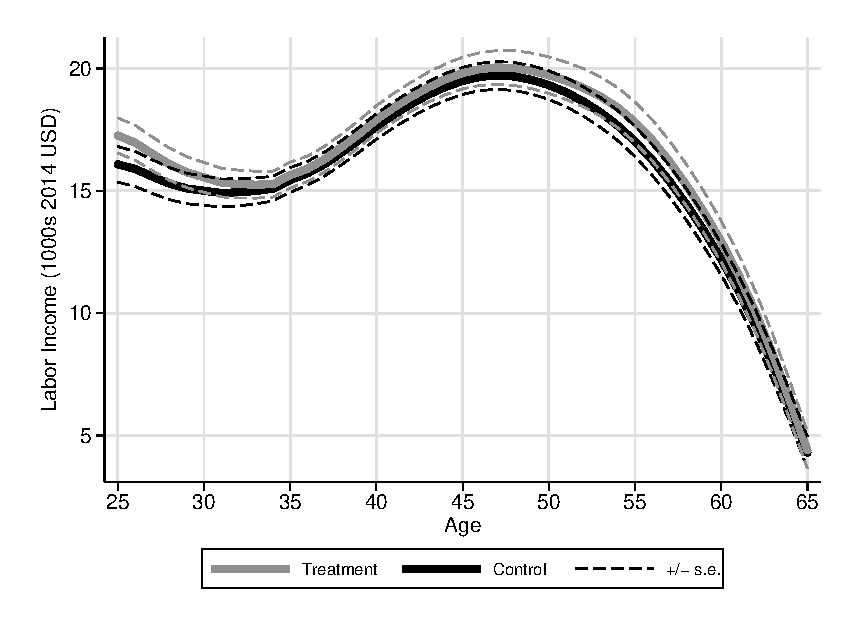
\includegraphics[width=\textwidth]{output/labor_25-60_female_4.eps}
\end{subfigure}%
\begin{subfigure}[h]{0.4\textwidth}
	\centering
	\caption{PSID, Disadvantaged Females} \label{fig:psid0}
		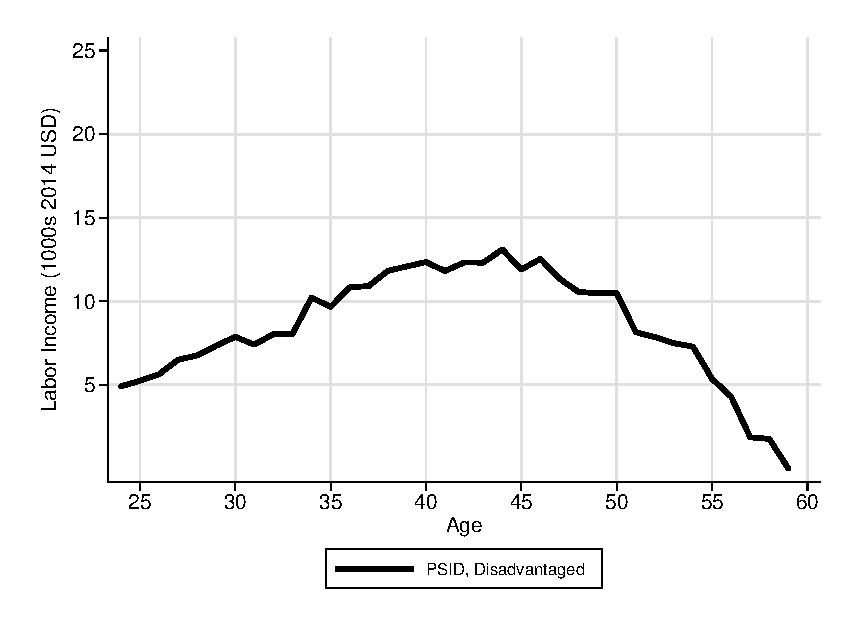
\includegraphics[width=\textwidth]{output/psid_incomeprofiles_s0.eps}
\end{subfigure}
\footnotesize \justify
Note: Panels (a) and (c) display the forecasted labor income profiles for ABC/CARE males and females by treatment status, based on forecasts that combine data from the Panel Study of Income Dynamics (PSID), the National Longitudinal Survey of Youth 1979 (NLSY79), and the Children of the National Longitudinal Survey of Youth 1979 (CNLSY79). Panels (b) and (d) display the mean labor income profile of disadvantaged males and females in the Panel Study of Income Dynamics (PSID), where disadvantaged is defined as having 12 years of education or less.\\
\end{sidewaysfigure}

\begin{sidewaysfigure}[!htbp]
\centering
\caption{Labor Income Profiles, Forecast Based on $W,Z$}\label{fig:labor-income-profiles}
\begin{subfigure}[h]{0.4\textwidth}
		\centering
		\caption{Forecasted for ABC/CARE Males} \label{fig:abcare1}
		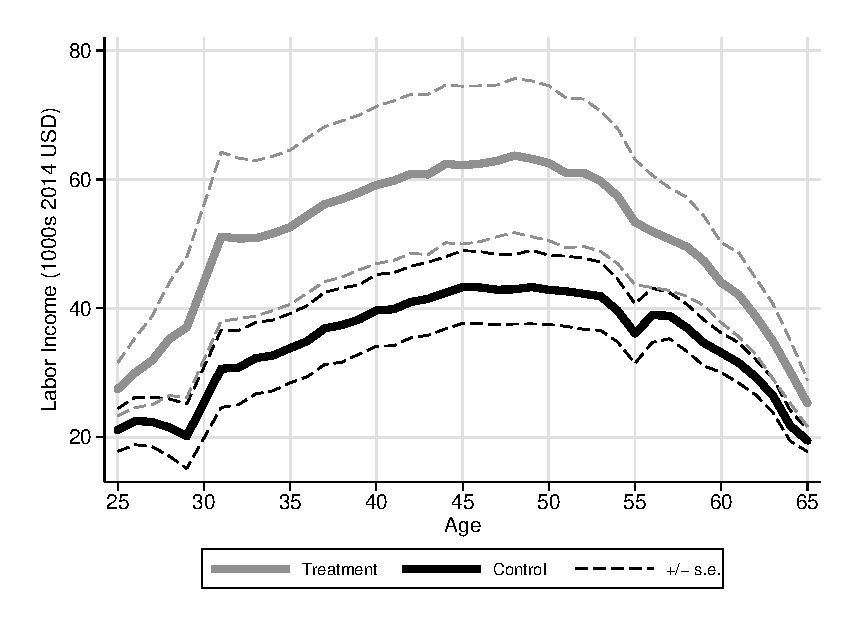
\includegraphics[width=\textwidth]{output/labor_25-60_male_5.eps}
\end{subfigure}%
\begin{subfigure}[h]{0.4\textwidth}
	\centering
	\caption{PSID, Disadvantaged Males} \label{fig:psid1}
		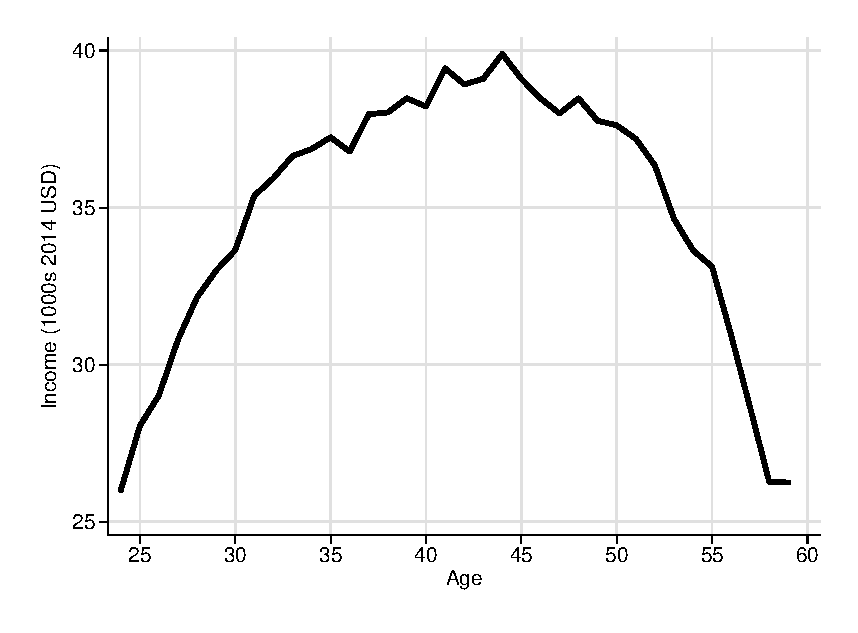
\includegraphics[width=\textwidth]{output/psid_incomeprofiles_s1.eps}
\end{subfigure}
\begin{subfigure}[h]{0.4\textwidth}
		\centering
		\caption{Forecasted for ABC/CARE Females} \label{fig:abcare0}
		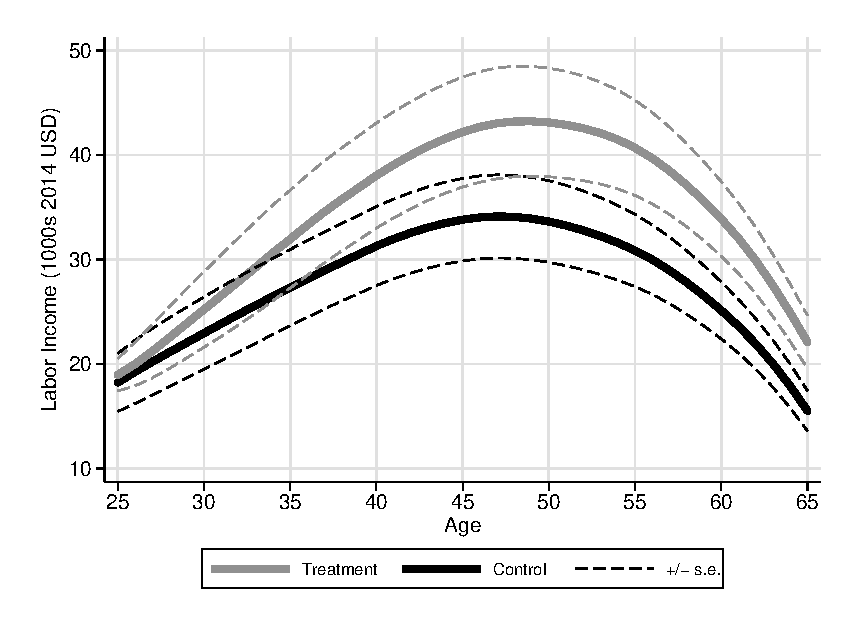
\includegraphics[width=\textwidth]{output/labor_25-60_female_5.eps}
\end{subfigure}%
\begin{subfigure}[h]{0.4\textwidth}
	\centering
	\caption{PSID, Disadvantaged Females} \label{fig:psid0}
		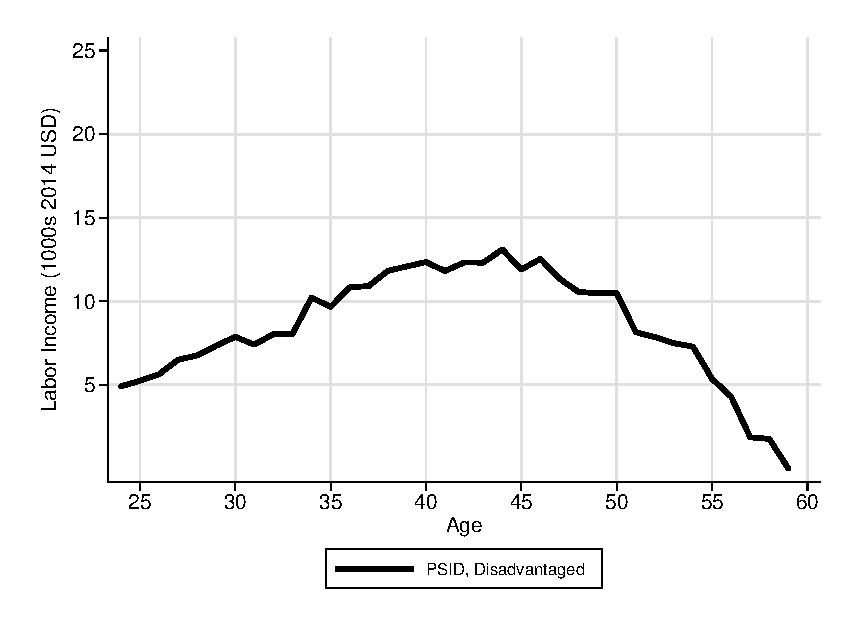
\includegraphics[width=\textwidth]{output/psid_incomeprofiles_s0.eps}
\end{subfigure}
\footnotesize \justify
Note: Panels (a) and (c) display the forecasted labor income profiles for ABC/CARE males and females by treatment status, based on forecasts that combine data from the Panel Study of Income Dynamics (PSID), the National Longitudinal Survey of Youth 1979 (NLSY79), and the Children of the National Longitudinal Survey of Youth 1979 (CNLSY79). Panels (b) and (d) display the mean labor income profile of disadvantaged males and females in the Panel Study of Income Dynamics (PSID), where disadvantaged is defined as having 12 years of education or less.\\
\end{sidewaysfigure}

\paragraph{Health Costs}

\noindent We predict health care costs from age 30 up to age 79, and criminal costs from birth
up to age 50. We then evaluate the predicted outcomes as if observed, and estimate the
treatment effect on those data.\\

\noindent As health outcomes are simulated using a set of variables exhibiting a high rate of attrition, the
predicted health outcomes exhibit an equal rate of attrition. We therefore employ the method described
in Appendix \ref{app:method_partialobs} to estimate the treatment effect on health care costs at
every age from 30 through 79, conditional on survival up to each age. \\

\paragraph{Crime Costs}

\noindent In the case of crime costs, we are able to predict costs for more than 100 individuals in the
sample. We therefore utilize the method described in Appendix~\ref{app:method_fullobs}
to estimate the treatment effect on the cost of criminal activity at every age from birth until age 50. \\

\subsection{Internal Rate of Return}
\label{app:method_irr}

\noindent To estimate the internal rate of return, we solve for $\rho$ in the equation below,

\begin{align}
\sum_{t=0}^T \frac{ \mathbb{E} (B_t - C_t)}{(1+\rho)^t} = 0,
\end{align}

\noindent where we let $T = 79$, define $B_t$ and $C_t$ to be the total benefits and costs of the program at time $t$, and define $\mathbb{E}(.)$ to be the sample mean. That is, we estimate the internal rate of return for the \textit{average subject} of ABC/CARE. \\

\noindent All outcomes of the parents and subjects that we observe as having been affected by the program are treated as benefits. For this to make sense, we reverse the sign of the monetized effect of the program on specific outcomes. Costs of ABC/CARE consist only of the initial program costs from ages 0 to 5. Table \ref{table:bc_comp} provides a full list of the benefits and costs of ABC. \\

\noindent We take the sum of the treatment effects on each component of the benefits to be the total benefit, $B_t$, of the ABC/CARE program. This includes parental income, subject labor income, and QALYs (quality-adjusted life years). Treatment effects on costs borne by the subject or society have their signs reversed and are included as benefits. We do this for subject public-transfer income, education costs, crime costs, control substitution costs, and health costs. To account for deadweight loss, we impose a marginal welfare cost of 50\% by multiplying public costs by a factor of $0.5$ when they are a direct transfer from the government to the individuals\footnote{There is no clear consensus on the marginal welfare cost of tax revenue. However, most researchers estimate the welfare cost per tax dollar to be between \$0.30 and \$0.50. See \citet{Feldstein_1999_REStat}, \citet{Heckman_Smith_1998_evaluating}, and \citet{Browning_1987_AER}.} When the public costs are not a direct transfer from the government to the individuals, we multiply them by a factor of $1.5$.\\

\noindent The principle for multiplying the public costs is the following. We evaluate the social benefits of ABC/CARE and do not place a value on who receives the money. The only social cost from a direct transfer is the dead-weight loss that it generates: $50\%$ of its total value. We do not consider education and criminal costs a direct transfer. Thus, we multiply them by a factor of $1.5$: the value of their cost plus $50\%$ of the value of their cost (the dead-weight loss implied in raising the public revenue to fund them). Table \ref{table:bc_comp} lists the factor we use to multiply each cost to account for its implied dead-weigh loss.\\

\noindent Having constructed our cash flow, $\mathbb{E} (B_t - C_t)$, solving for $\rho$
reduces to an algebraic exercise.\\

\noindent We estimate the treatment effect on each
component of the benefits and costs at time $t$ for the pooled, male, and
female samples. We do this for 1,000 bootstrap resamples of the original ABC/CARE data.
In the case of health costs and subject income, for which we employ auxiliary datasets to
estimate the treatment effects, we also obtain 1,000 bootstrap estimates from the auxiliary data
for every ABC/CARE bootstrap resample, resulting in a total of 1,000,000 estimates.
By reusing each bootstrap estimate of the treatment effect on outcomes that do not require any auxiliary data
set 1,000 times, we obtain a total of 1,000,000 estimates of the cash flow.
We estimate the internal rate of return on each of those cash flows.
This is how we form our empirical bootstrap distribution of the internal rate of return for the pooled, male, and female samples.
We take the mean of the distributions to be the point estimates, and we take the standard deviations
to be the standard errors. To construct the 80\% confidence intervals, we take the 10\textsuperscript{th}
and 90\textsuperscript{th} quantiles of each bootstrap distribution. \\

% We let $T = 79$. In Appendix \ref{app:method_identify}
% we explain how we can estimate the summand of the numerator at every period $t$, which
% can be expressed as $\mathbf{E}(B_t) -  \mathbf{E}(C_t)$. Thus, solving for $\rho$
% reduces to an algebraic exercise.



% To construct our cash flow, we subtract the costs from benefits to create a single stream.
% We define `cost' to include only the program costs of ABC, and define
% `benefits' to include all treatment effects of the program. This includes
% the treatment effects on parent income, subject labor income, and QALY
% (quality adjusted life years).\footnote{QALYs are measured on a scale of 0 to 1, with 1 being a
% year of perfect health. We follow \textbf{[CITATION]} and value a QALY of 1 to be
% \$150,000, and a QALY of 0 to be \$0. The dollar value of that year relates linearly to the QALY.}
% Treatment effects on costs borne by the subject or society have their signs
% reversed and are included as benefits. We do this for subject transfer income,
% education costs, jail costs, justice system costs, victimization costs,
% control contamination costs, and medical costs. To account for deadweight loss, we
% impose a marginal welfare cost of 50\% by multiplying public costs by a factor of
% $1.5$.\footnote{There is no clear consensus on the marginal welfare cost of tax revenue. However,
% most researchers estimate the welfare cost per tax dollar is between \$0.30--0.50. See
% \citet{feldstein1999tax, heckman1998evaluating, browning1987marginal}.} This
% includes education cost up until age 17, jail costs, justice system costs, Medicare costs,
% and Medicaid costs. For the same reason, we multiply transfer income by a factor of 0.5.

% For each period $t \in \{1, 2, \dots, 79\}$, we sum our estimates of the benefits, and
% subtract our estimates of the costs from that sum. This provides us an estimate of
% $\mathbf{E}(B_t) -  \mathbf{E}(C_t) = \mathbf{E} (B_t - C_t)$. We then solve for
% $\rho$ using numerical analysis.

% In your methodlogy you describe costs and benefits differnetly....
% To construct our cash flow, we sum the costs and benefits from the program into a single stream.
% We define `cost' to include only the cost of implementing ABC. On the other hand,
% we broadly define `benefits' to include all treatment effects of the program. This includes
% the treatment effects on parent income, subject labor income, and QALY
% (quality adjusted life years).\footnote{QALYs are measured on a scale of 0 to 1, with 1 being a
% year of perfect health. We follow \textbf{[CITATION]} and value a QALY of 1 to be
% \$150,000, and a QALY of 0 to be \$0. The dollar value of that year relates linearly to the QALY.}
% Treatment effects on outcomes generally considered to be costs have their signs reversed in
% order to convert them into benefits. We do this for subject transfer income,
% education costs, jail costs, justice system costs, victimization costs,
% control contamination costs, and medical costs. To account for deadweight loss, we
% impose a marginal welfare cost of 50\% by multiplying public costs by a factor of
% $1.5$.\footnote{There is no clear consensus on the marginal welfare cost of tax revenue. However,
% most researchers estimate the welfare cost per tax dollar is between \$0.30--0.50. See
% \citet{feldstein1999tax, heckman1998evaluating, browning1987marginal}.} This
% includes education cost up until age 17, jail costs, justice system costs, Medicare costs,
% and Medicaid costs. For the same reason, we multiply transfer income by a factor of 0.5.


\subsection{Computing the Benefit/cost Ratio}
\label{app:method_cbratio}

\noindent The benefit/cost ratio can be expressed as,

\begin{align}
\mathbb{E} \left( \frac{ \sum_{t=0}^T B_t}{\sum_{t=0}^T C_t} \right),
\end{align}

\noindent where we let $T = 79$, define $B_t$ and $C_t$ to be the total benefits and costs of the
program at time $t$, and define $\mathbb{E}(.)$ to be the sample mean. See Table \ref{table:bc_comp} for a detailed list of the components
to the benefits and costs of ABC/CARE . We take the sum of the treatment effects on each component
of the benefits to be the total benefits of the ABC/CARE programs. \\

\noindent To account for deadweight loss, we assume a marginal welfare cost of 50\% by multiplying
public costs components by a factor of $1.5$. For the same reason, we multiply public-transfer
income by a factor of 0.5. We discount each component of the benefits and costs
by 3\% every year to obtain their net present value at birth. We then sum up the discounted
components of the benefits and find the ratio with the discounted costs. \\

\noindent We estimate the treatment effect on each
component of the benefits and costs at time $t$ for the pooled, male, and
female samples. We do this for 1,000 bootstrap resamples of the original ABC/CARE data.
In the case of health and subject income, for which we employ auxiliary datasets to
estimate the treatment effects, we also obtain 1,000 bootstrap estimates from the auxiliary data
for every ABC/CARE bootstrap resample, resulting in a total of 1,000,000 estimates.
By reusing each bootstrap estimate of the treatment effect on outcomes that do not require any auxiliary data
set 1,000 times, we obtain a total of 1,000,000 estimates of the costs stream and benefits stream.
We estimate the benefit/cost ratio for each of those streams.
This is how we form our empirical bootstrap distribution of the benefit/cost ratio for the pooled, male, and female samples.
We take the mean of the distributions to be the point estimates, and we take the standard deviations
to be the standard errors. To construct the 80\% confidence intervals, we take the 10\textsuperscript{th}
and 90\textsuperscript{th} quantiles of each bootstrap distribution.

\begin{table}[H]
\begin{threeparttable}
\caption{Components of Benefits and Costs}
\label{table:bc_comp}
\centering
\begin{tabular}{l c c}
\toprule			
Variable & Sign Reversed	& Welfare Cost \\
	&		& Factor \\
\midrule
\textbf{Benefits} 	\\			
\quad Parent Income			& \\
\quad Subject QALY			& \\
\quad Subject Labor Income	& \\
\quad Subject Public-transfer Income	& $\checkmark$	& 0.5 \\
\quad Medicare Costs			& $\checkmark$	& 1.5 \\
\quad Medicaid Costs			& $\checkmark$	& 1.5 \\
\quad Out-of-pocket Medical Costs	& $\checkmark$ \\
\quad Miscellaneous Medical Costs	& $\checkmark$ \\
\quad Disability Insurance Claim	& $\checkmark$	&	1.5 \\
\quad Social Security Claim	& $\checkmark$	&	1.5 \\
\quad Supplemental Security Claim	& $\checkmark$	&	1.5 \\
\quad Control Substitution Costs	& $\checkmark$	& \\
\quad Education Costs			& $\checkmark$	& 1.5* \\
\quad Justice System Costs	& $\checkmark$	& 1.5 \\
\quad Prison Costs			& $\checkmark$	& 1.5 \\
\quad Victimization Costs		& $\checkmark$	& \\
\textbf{Costs} 	\\			
\quad Program Costs			& \\
\bottomrule			
\end{tabular}
\begin{tablenotes}
\footnotesize
\item Note: The table lists the components of the costs and benefits of ABC/CARE.
In order for some components to be categorized as benefits, we reversed the sign
of the treatment effect. *Only education costs up until age 18 are multiplied by 1.5 to account for welfare costs. This factor is drawn from \citet{Heckman_Moon_etal_2010_RateofReturn}.
\end{tablenotes}
\end{threeparttable}
\end{table}


